% !TeX root = ../../thesis.tex
\chapter{Model applications: patient-specific porous acetabular implants}\label{ch:cup}

\begin{shaded}
This chapter is based on a manuscript prepared to be submitted:\\
M. Barzegari, F. Perez-Boerema, G. Zavodszky, and L. Geris, ``High-performance computer simulation of biodegradation of optimized personalized implants; a case study of a patient-specific porous acetabular implant.''
\end{shaded}

In this chapter, the developed biodegradation work is tested on the output of a surrogate model for design optimization of patent-specific orthopedics implants, which can be seen as coupling of the two models. Since the output of the surrogate model has a high level of geometrical details, the corresponding biodegradation model becomes highly computational-intensive, making it suitable for tuning and evaluating the HPC scaling behavior of the model.

\section{Introduction}

\newglossaryentry{THA}{name={THA},description={total hip arthroplasty}}

3D-printed orthopedic implants have been gaining popularity in recent years due to this manufacturing technique giving the designer control over the different design aspects of the implant \cite{Kumar2021,Yadav2020}. It allows manufacturing implants with specific designs and using material properties similar to the bone, allowing the implant designer to address complications experienced in various surgeries such as total hip arthroplasty (\gls{THA}). The implants used in \gls{THA} consist of three main components: a femoral stem, a liner and an acetabular component, which comprises a cup and a solid (or porous) part on top. In large bone defects and severe deformations, the acetabular component can be designed and made patient-specific, an example of which is shown in Fig. \ref{fig:cup_implant_real} (Ortho Baltic Implants Co., Lithuania). This patient-specific design has certain advantages such as decreased mechanical instability risk, adaptation of the implant shape to the patient's bone geometry, restoring the biomechanics of the joint after the severe fractures, and optimal positioning of the screws.

\begin{figure}[htpb]
\centering
\medskip
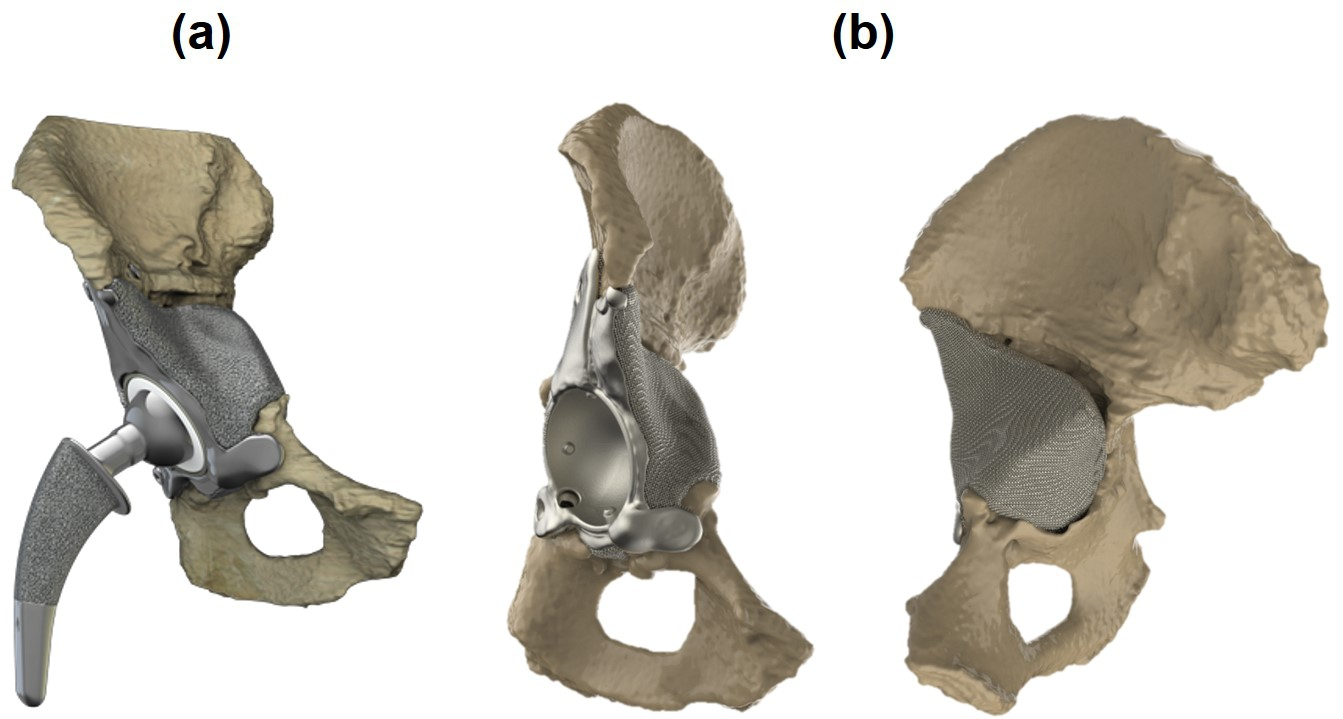
\includegraphics[width=\textwidth]{implant_real.jpg}
\caption[Full setup of patient-specific acetabular implants]{Demonstration of patient-specific acetabular implants in large bone defects (reproduced with permission from Ortho Baltic Implants Co.\protect\footnotemark), a) the full setup comprises of a femoral stem, a liner and an acetabular component, b) a sample design of the acetabular component which consists of a (non-degradable) cup and a porous part designed to match the geometry of the patient's fractured bone. The porous part can be manufactured from biodegradable materials such as Mg alloys.} \label{fig:cup_implant_real}
\end{figure}

Although such a patient-specific design helps surgeons address multiple problems in the first place, other issues may emerge during revision surgeries, an example of which is the aseptic loosening of the implant after \gls{THA}. The rate and quality of bone regeneration after implantation of orthopedic implants depends significantly on the achieved (initial and long-term) mechanical stability. To restore proper function after the implant loosening, the implant needs to be replaced. During these revision surgeries, some bone is removed along with the implant, further increasing the already present bone defects and making it harder to achieve proper mechanical stability with the revision implant \cite{Luthringer2014}. A possible way to limit the increasing loss of bone is using (partially) biodegradable orthopedic implants that optimize long-term implant stability, in which part of the implant, like the irregular patient-specific part on top of the acetabular cup in Fig. \ref{fig:cup_implant_real}, is made from biodegradable metals. This means that the biodegradable part of the implant will disappear and be replaced by newly formed bone during the implant's lifetime. Taking advantage of these implants needs to optimize the implant so that stress shielding is minimized and tune the implant degradation rate so that newly formed bone can replace the degrading metal to maintain proper bone-implant contact. The hope is that such (partly) degradable implants will lead to a reduction in the size of the bone defects over time, making possible future revisions less likely and less complex.

\footnotetext{\url{https://balticimplants.eu/}}

In this study, we focused on improving the long-term implant stability of patient-specific acetabular implants for large bone defects and tuning their biodegradable behavior. To improve the long-term implant stability, a surrogate-based optimization approach was implemented that sought to reduce implant-induced stress shielding by adjusting the stiffness of an acetabular implant. The optimized stiffness was subsequently translated into a porous implant design of varying porosity. In the initial stage of developing a computational workflow containing both the patient-specific optimization routine and the biodegradation model, the geometry of the acetabular component of the implant was assumed to be only the cup by ignoring the additional parts on top, all of which is designed to be porous and made from biodegradable materials (Fig. \ref{fig:cup_implant}). Although this assumption was made for demonstration purposes and simplifying the geometry of the optimization model, the workflow can be applied to the full acetabular implant setup consisting of a cup-shaped non-degradable part (combined with a polyethylene cup) and a patient-specific porous degradable part matching the patient's bone geometry in the future.

\begin{figure}[h]
\centering
\medskip
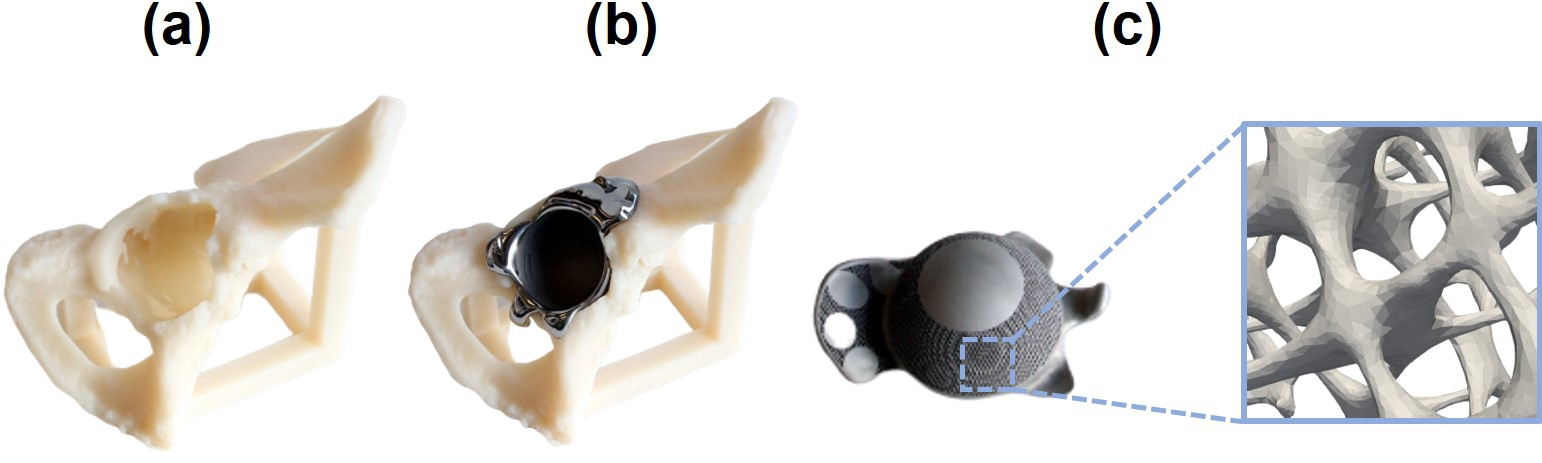
\includegraphics[width=\textwidth]{implant.jpg}
\caption[Demonstration of the simplified patient-specific acetabular implant]{Demonstration of the simplified patient-specific acetabular implant used in the current study to demonstrate the developed computational workflow, which assumed to have a porous structure on its back made from biodegradable metals, a) the large bone defects in the hip bone, b) the implant used for fixing the problem in the total hip arthroplasty surgery, c) the porous structure on the back of the implant, which is assumed to be biodegradable for demonstration purposes. This part is made from non-degradable materials in real-case scenarios to provide support to the patient-specific degradable part attached to it (Fig. \ref{fig:cup_implant_real}). Polyethylene liner not shown.} \label{fig:cup_implant}
\end{figure}

A quantitative mathematical model of the degradation process is a useful tool for tuning the biodegradation and material release rate, allowing researchers to study the biodegradation behavior of any desired implant \textit{in silico} (in the computer) prior to conducting any \textit{in vitro} or \textit{in vivo} experiments. Developed mathematical models can be simulated using efficient numerical schemes such as the finite element method. The primary challenge here will be achieving a high numerical accuracy at the interface between the implant and surrounding tissue in the body since the interface plays an important role in the degradation phenomena. Increased accuracy means increased computational cost and resources (especially time), but high-performance computing (\gls{HPC}) techniques can be used to overcome this challenge.

The implant design optimization (surrogate-based and topology optimization) is the PhD work of Fernando Perez-Boerema (in preparation), that is extended in this chapter with a model of the metal biodegradation process. Hence, the focus of the description here will be on the coupling with the degradation module as well as the improvement of the use of HPC techniques.


\section{Materials and methods}

\subsection{Surrogate-based optimization model}

\newglossaryentry{PCA}{name={PCA},description={principal component analysis}}
\newglossaryentry{RBF}{name={RBF},description={radial basis function}}

Two patient-specific finite elements (FE) models of the hip joint, i.e., one with implant and one without, were derived from computed tomography (\gls{CT}) scans of the pelvis, implemented using MARC/MENTAT software (Perez-Boerema et al., in preparation). The elastic modulus of the implant was parametrized, making use of two paraboloids, one for the upper half of the acetabular implant and one for the lower half. The FE model of the hip joint with implant was then used to generate a surrogate model by first applying a principal component analysis (\gls{PCA}) in order to reduce the size of the output space and subsequently constructing a radial basis function (\gls{RBF}) surrogate, implemented in MATLAB. The resulting surrogate model was used in a multi-start local optimization routine that relied on sequential quadratic programming to perform the local optimizations. The optimization had as objective minimizing the difference in stresses between the physiological control (no implant) and the case with implant. The coefficients of the paraboloids used to parametrize the elastic modulus were taken to be the design variables. The elastic modulus was limited to values between 1.2 and 110 GPa, while implant stresses were constrained to at most 0.3 times the yield stress. The optimized stiffness distribution was subsequently used to design an acetabular implant with a local porosity chosen to match the optimized global stiffness distribution. To this end, the open-source tool ASLI \cite{Perez-Boerema2022} was developed in-house, facilitating the generation of a skeletal-gyroid-based infill of varying porosity that can be tuned to match a predefined (in this case, the optimized) stiffness.

\subsection{Biodegradation model}

In this application chapter, we apply the previously developed quantitative mathematical model capturing the biodegradation of magnesium-based implants (Chapter \ref{ch:core}). Magnesium (Mg) was selected to start with due to its acceptable mechanical properties, biocompatibility, and contribution to osteoinductivity \cite{Agarwal2016}. The developed model captures the release of Mg ions, the formation of a protective film,  the dissolution of this film due to the presence of various ions in the surrounding environment, and the change in pH. This was accomplished by deriving a system of nonlinear time-dependent reaction-diffusion partial differential equations (\gls{PDE}s) from the underlying oxidation-reduction reactions occurring during the biodegradation process of metallic materials in simulated body fluid. The level-set formalism was employed to track the movement of the biodegradation front between the implant and its surroundings. The equations were solved implicitly using the finite element method for spatial terms (with a 1st order Lagrange polynomial as the shape function) and backward-Euler finite difference method for temporal terms on an Eulerian mesh, implemented in the open-source \gls{PDE} solver FreeFEM \cite{Hecht2012}. The details of this model can be found in Chapter \ref{ch:core} and  \cite{Barzegari2021}. Two separate simulations were performed using two different diffusion coefficients, as calibrated in our previous work, to model the degradation behavior in non-buffered and buffered solutions.

In order to build the computational model, the resulting surface mesh of the surrogate-based optimization routine, consisting of \num{5347924} faces, was converted to a volume mesh and embedded in a cubic container that was to act as the environment during the biodegradation simulations. The conversion of the surface mesh was performed using GMSH \cite{Geuzaine2009}, and the embedding process was carried out using the internal mesh engine of FreeFEM, called BAMG. The mesh was refined on the implant-environment interface to increase the numerical accuracy of the interface tracking model, leading to a final mesh with \num{45870053} elements. The mesh refinement process was handled using Mmg \cite{Dapogny2014} (and ParMmg \cite{balarac:hal-03344779}). Fig. \ref{fig:cup_model} shows the embedded cup model and a cross-section of the final generated mesh, which was refined on the metal-solution interface.



\begin{figure}[h]
\centering
\medskip
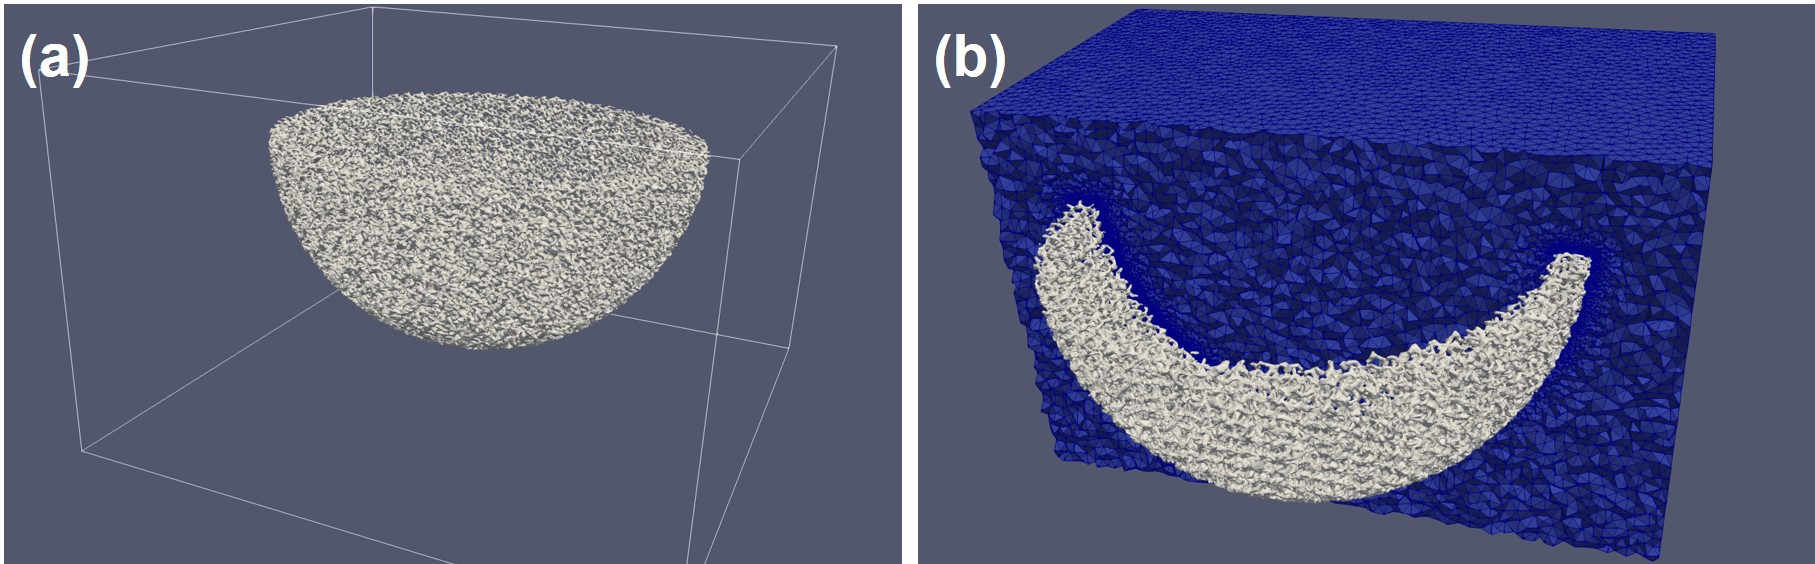
\includegraphics[width=\textwidth]{model.jpg}
\caption[Computational biodegradation model for the porous acetabular implant]{The computational biodegradation model for the porous acetabular implant: a) the optimized acetabular implant embedded inside a cubic container, b) a cross-section of the generated mesh with the implant's surface visualized as the light gray surface.} \label{fig:cup_model}
\end{figure}

For dealing with a problem of this size and making the model capable of being scaled in large-scale computing systems, the model implementation made use of the \gls{HPC} techniques available in the FreeFEM language v4.10 and \gls{PETSc} toolkit v3.16.1 \cite{petsc}. In this implementation, METIS and ParMETIS graph partitioners \cite{METIS1998} were used to decompose the mesh into various partitions, and then the partitioned mesh was distributed among available computing resources using the \gls{HPDDM} preconditioner \cite{Jolivet2013}. Fig. \ref{fig:cup_decomposition} shows the decomposition of the computational mesh. Moreover, the HYPRE BoomerAMG \cite{Falgout2002} preconditioner and \gls{GMRES} iterative solver \cite{Saad1986} were used to solve the linear systems of equations obtained from applying the finite element discretization on the model. More details of the implementation can be found in Chapter \ref{ch:hpc} and \cite{Barzegari2022}.

\begin{figure}[h]
\centering
\medskip
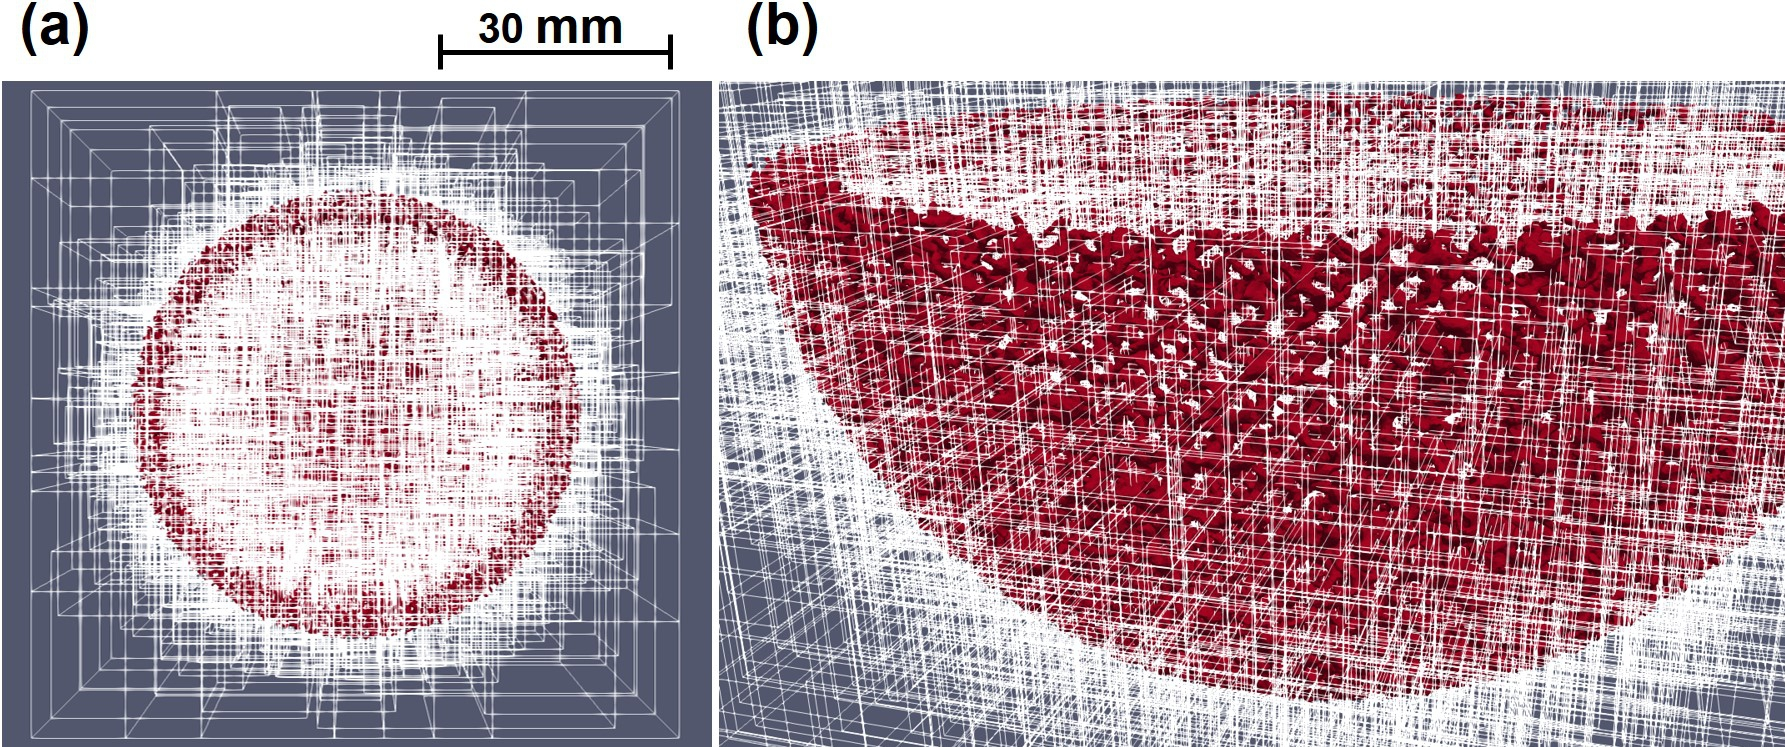
\includegraphics[width=\textwidth]{decomposition.jpg}
\caption[Mesh decomposition of the acetabular implant model]{Mesh decomposition of the computational biodegradation model to be distributed to available computing nodes, a) top view, b) perspective side view. } \label{fig:cup_decomposition}
\end{figure}

The simulation was carried out using 2,000 \gls{CPU} cores with 16.5 TB of available memory on the Dutch national supercomputer, Snellius. The simulation results, comprising of \num{95000} files with a total size of 148 GB, were visualized using a parallel client-server remote rendering approach in ParaView server v5.9.1 running on 128 \gls{CPU} cores on the ARCHER2 supercomputer.

In order to obtain the scaling behavior of the model in an \gls{HPC} environment, strong and weak scaling tests were performed on the Snellius supercomputer. For the weak scaling test, in addition to the mesh with \num{45870053} elements, two more mesh files consisting of fewer elements were generated using the aforementioned procedure for embedding and refining the mesh. These models had \num{15989521} and \num{29035491} tetrahedral elements, respectively, to which the number of employed \gls{CPU} cores was adjusted accordingly. The strong scaling test was carried out for all three model sizes by varying the number of employed \gls{CPU} cores from 60 to \num{9000}.


\section{Results and discussion}

\subsection{Surrogate-based optimization of the acetabular implant}

The optimized design to minimize stress shielding, depicted in Fig. \ref{fig:cup_optimization},  has a skeletal-gyroid infill of varying porosity with apparent elastic moduli ranging from 4.7 to 49 GPa and an estimated acetabular stress shielding reduction of about 56\% compared to a solid titanium implant.

\begin{figure}[h]
\centering
\medskip
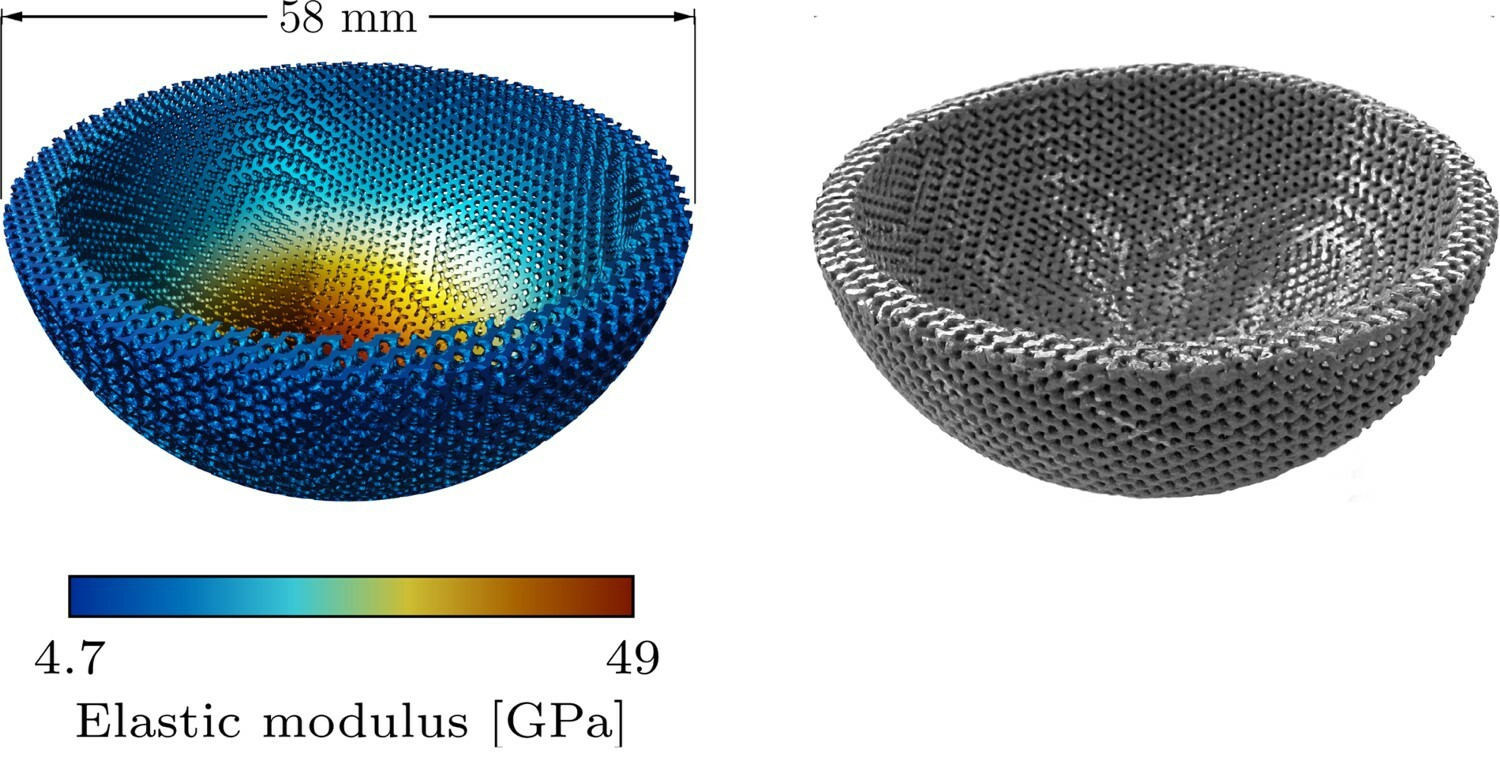
\includegraphics[width=\textwidth]{optimization.jpg}
\caption[Acetabular implant infilled by skeletal gyroid microstructure with varying volume fraction]{Titanium acetabular implant infilled by skeletal gyroid microstructure with varying volume fraction to match a desired apparent stiffness distribution  \cite{Perez-Boerema2022}}. \label{fig:cup_optimization}
\end{figure}

The varying porosity was adjusted during a surrogate-based optimization process to match the stiffness distribution required to minimize stress shielding during the bone healing process. Considering the target application is bone tissue engineering, the infill used to generate the lattice structure was selected based on triply periodic minimal surfaces (\gls{TPMS}). \gls{TPMS}-based lattices have shown good performance for biological processes of cell attachment, migration, and proliferation \cite{RAJAGOPALAN2006,Hede2021}, making them a suitable choice for tissue engineering applications where their aim is to guide tissue growth. This positive influence is routed in the appropriate balance of various structural and mechanical properties required to improve bone tissue formation, such as yield strength, fatigue strength, adequate mechanical stimulus, and permeability \cite{OtextquotesingleBrien2011,Hollister2005}.

\subsection{Biodegradation of the infilled implant}

Fig. \ref{fig:cup_degradation_rate} shows the mass loss during the biodegradation for simulations performed in buffered (low degradation rate) and non-buffered (high degradation) solutions. Mass loss is one of the commonly-used indicators for the degradation rate, demonstrating that the biodegradation rate is much higher in the non-buffered solution. Although evaluated on different geometries with certain effect on the results, loss of material over time was found to be comparatively in line with the values obtained in Chapter \ref{ch:core} and \cite{Barzegari2021}, with the mass loss in the saline solution being 6 to 10 times more than that of buffered solution in evaluated time points before 21 hours.  It shows that scaling the model in an \gls{HPC} environment does not affect the quantitative predictions made by the model. The developed mechanistic model of the biodegradation process includes a level-set equation correlating the loss of material to the velocity at which the implant interface shrinks. The aforementioned agreement of results on a large scale (a model with $\sim$45M elements) shows that the interface tracking formulation behaves efficiently even in problems with a high level of details. This verifies the performance of the developed biodegradation model, which has never been tested before in such high resolutions.

\begin{figure}[h]
\centering
\medskip
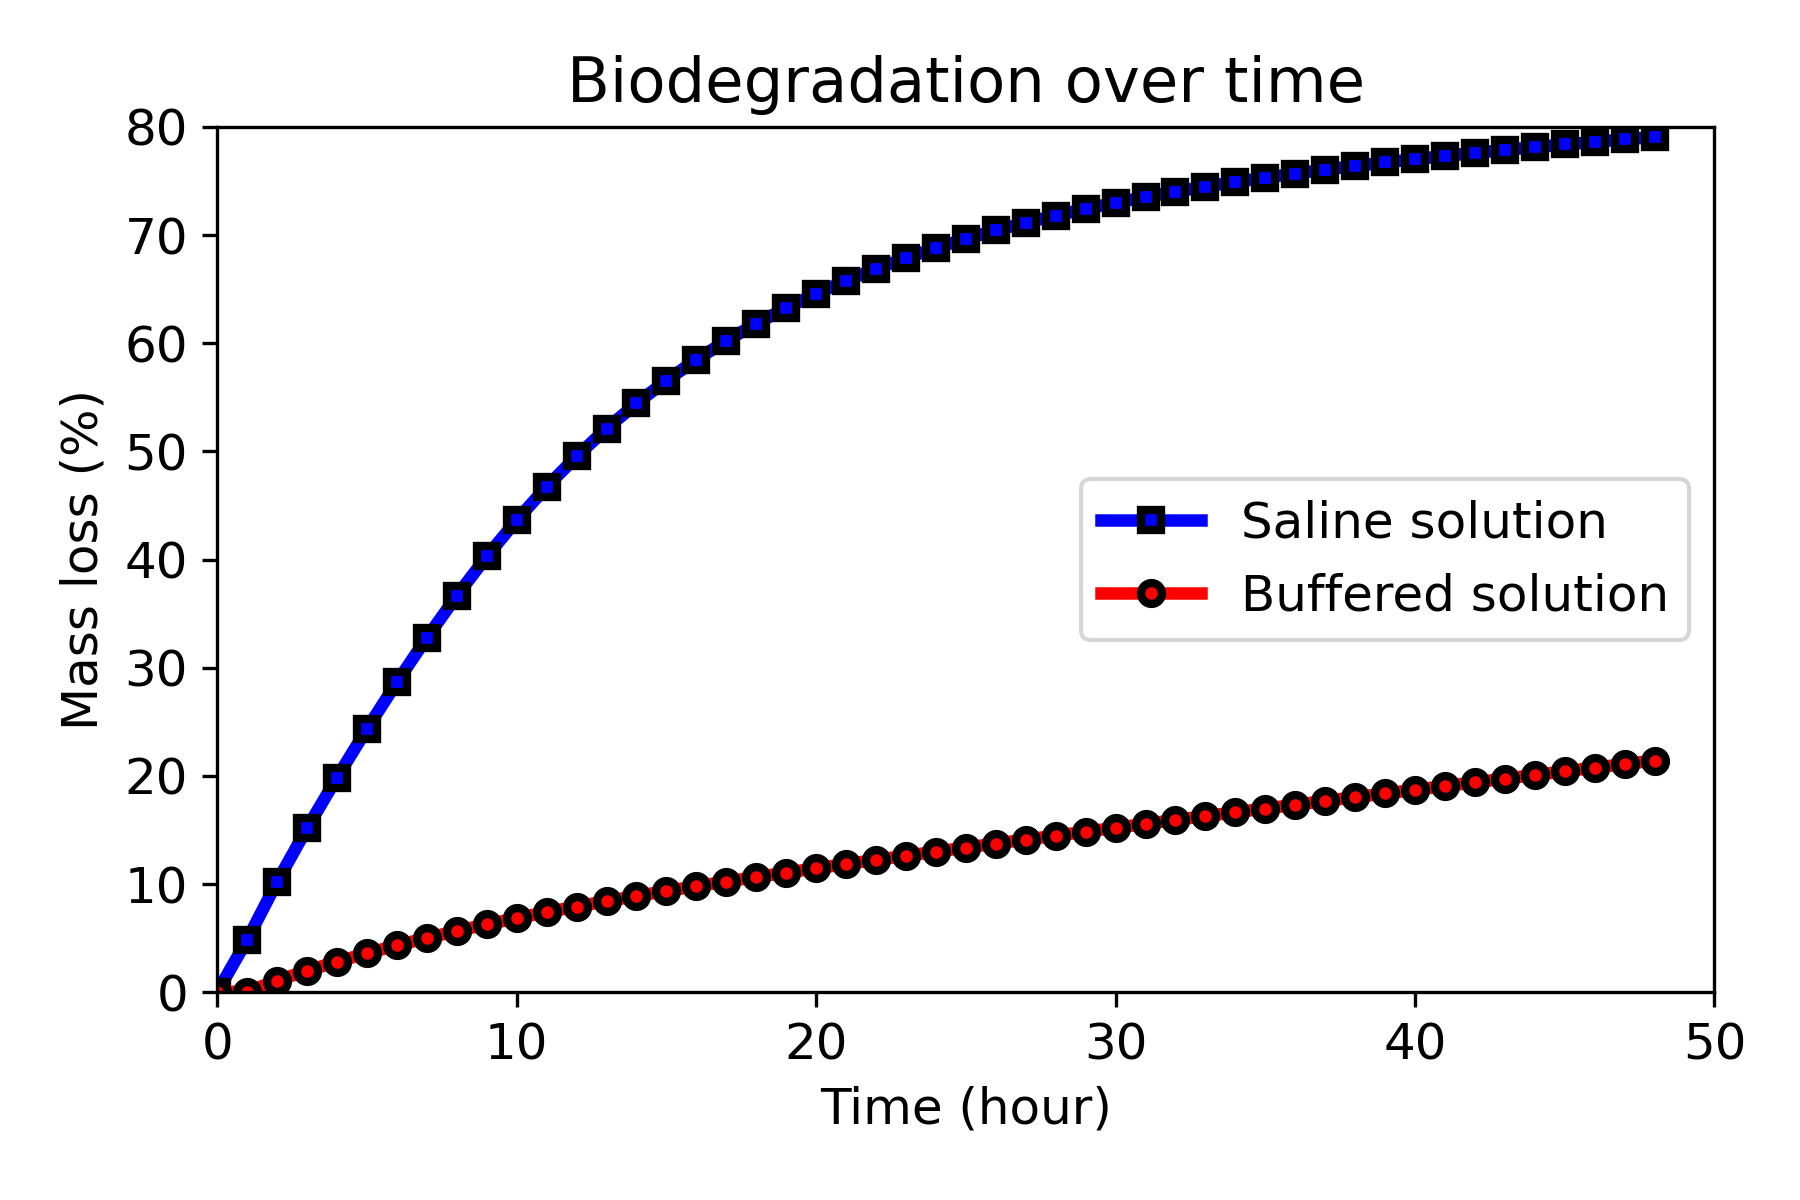
\includegraphics[width=0.7\textwidth]{degradation_rate.png}
\caption[Biodegradation rate for the acetabular implant]{Rate of mass loss during the biodegradation of the porous acetabular implant in saline and buffered solutions.} \label{fig:cup_degradation_rate}
\end{figure}

From a qualitative point of view, visualizing the biodegradation results over time, depicted in Fig. \ref{fig:cup_degradation_visual}, shows that the acetabular implant degrades faster in the regions with higher porosity, i.e., the regions with more exposed surface area to the environment. These are the regions designed to have lower stiffness, resulting in high porosity after being filled with \gls{TPMS} unit cells with a lower volume fraction. From the induced bone formation perspective, the implant parts with low stiffness disappear during the bone healing process, a fact that can be further taken into account in the optimization procedure.
%This correlation can also be discussed from the pathological perspective, meaning that the parts with low stiffness get replaced faster by the newly formed bone during the bone healing process. It is the expected behavior of the porous implant and the aim of such a patient-specific design.

\begin{figure}[h]
\centering
\medskip
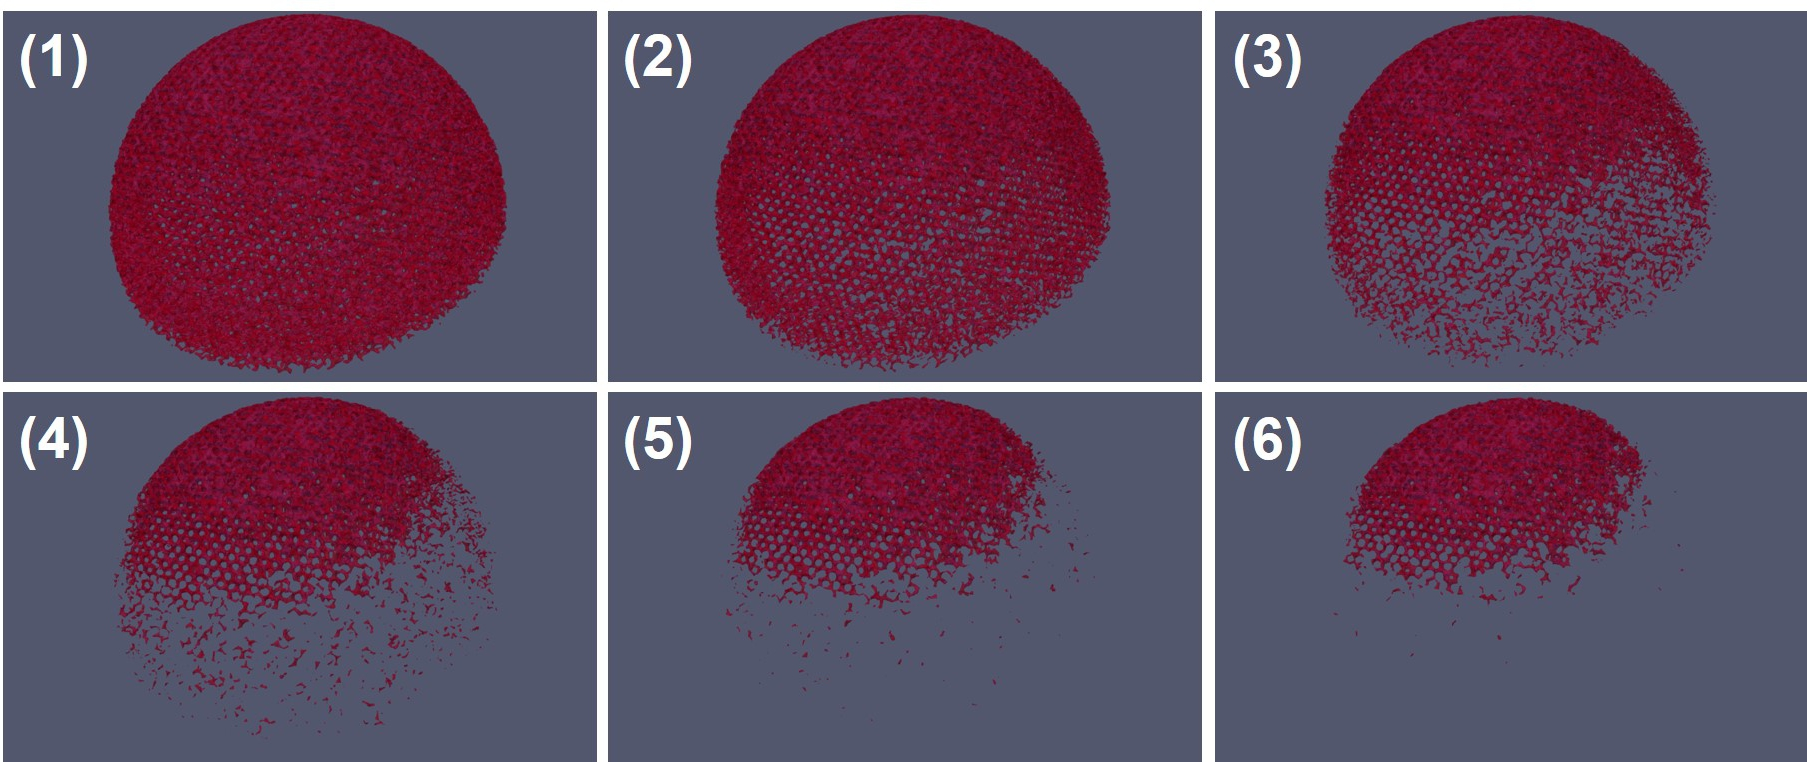
\includegraphics[width=\textwidth]{degradation_visual.jpg}
\caption[Visualization of the change of morphology of the acetabular implant]{Visualization of the change of morphology of the acetabular implant over time (1) to (6).} \label{fig:cup_degradation_visual}
\end{figure}

Fig. \ref{fig:cup_degradation_visual_close} demonstrates a similar visualization but with a zoomed view on the surface of the implant being plotted along with a cross-section of the medium showing the concentration of released Mg ions. The movement of the corrosion interface is formulated based on the release of material ions, and as a result, the material loss rate is higher in regions with higher ions concentration. The concentration is directly correlated to the exposed surface area, meaning that a higher surface-to-volume ratio results in a higher material release. This explains why the regions with higher porosity degrade faster in the current biodegradation model.%, which turns out to be a realistic behavior captured correctly by the developed mathematical model.

\begin{figure}[h]
\centering
\medskip
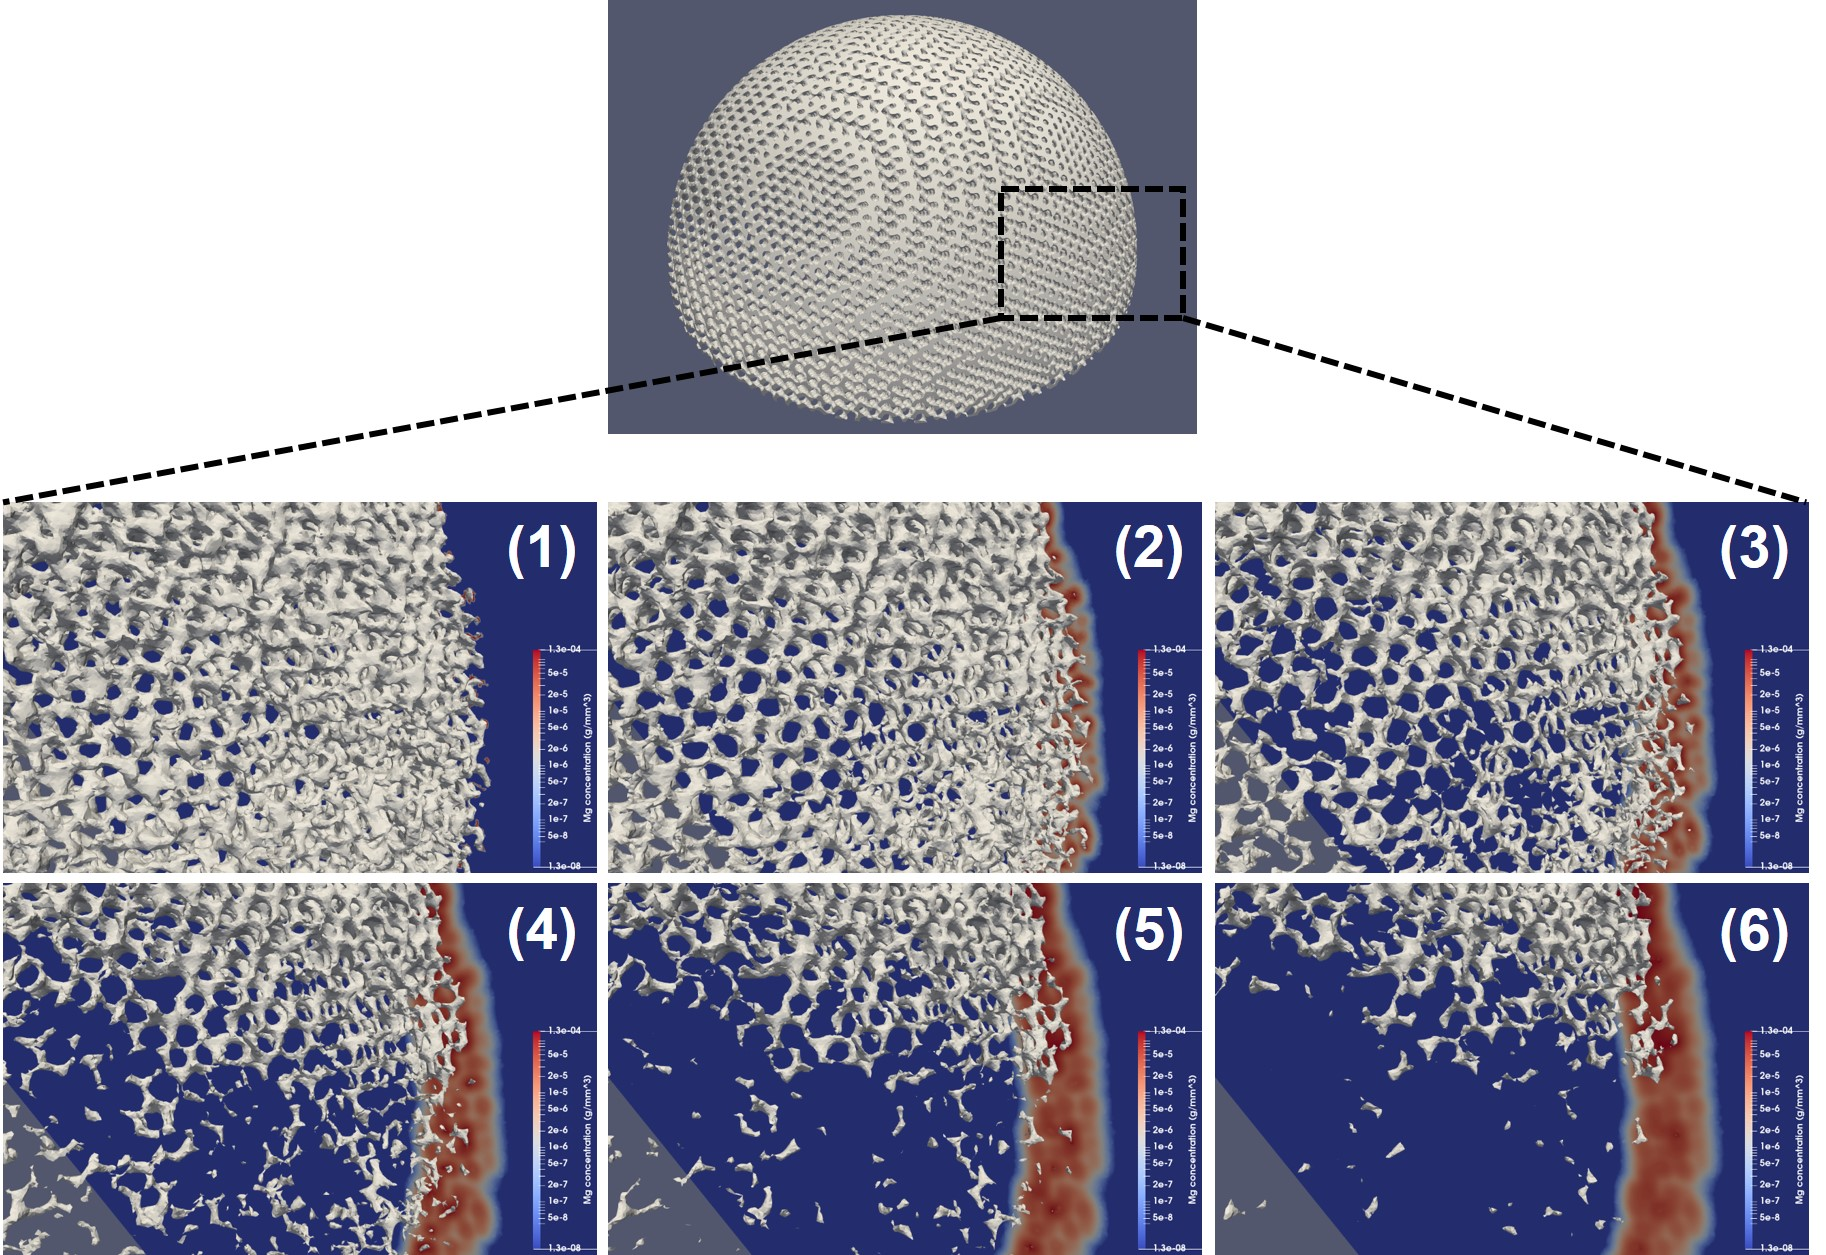
\includegraphics[width=\textwidth]{degradation_visual_close.jpg}
\caption[Visualization of the change of morphology of the acetabular implant]{A closer look at the visualization of the change of morphology of the acetabular implant over time ((1) to (6)) along with a cross-section of the medium showing the concentration of released Mg ions.} \label{fig:cup_degradation_visual_close}
\end{figure}

\subsection{Scaling tests on the computational models}

The results of the strong scaling tests are plotted in Fig. \ref{fig:cup_strong_scaling}, which shows the solution time of individual equations of the biodegradation model in a single time step versus the varying number of \gls{CPU} cores. The comprising equations are the transport equation for Mg ions (Mg equation), hydroxide ions (OH equation), and chloride ions (Cl equation), as well as the film formation (film equation) and the derived level-set equation. These equations are detailed in Chapter \ref{ch:core} and \cite{Barzegari2021}. The run time of a single time step was measured for three model sizes of $\sim$16M (small), $\sim$29M (medium), and $\sim$45M (big) elements.

\begin{figure}[h]
\centering
\medskip
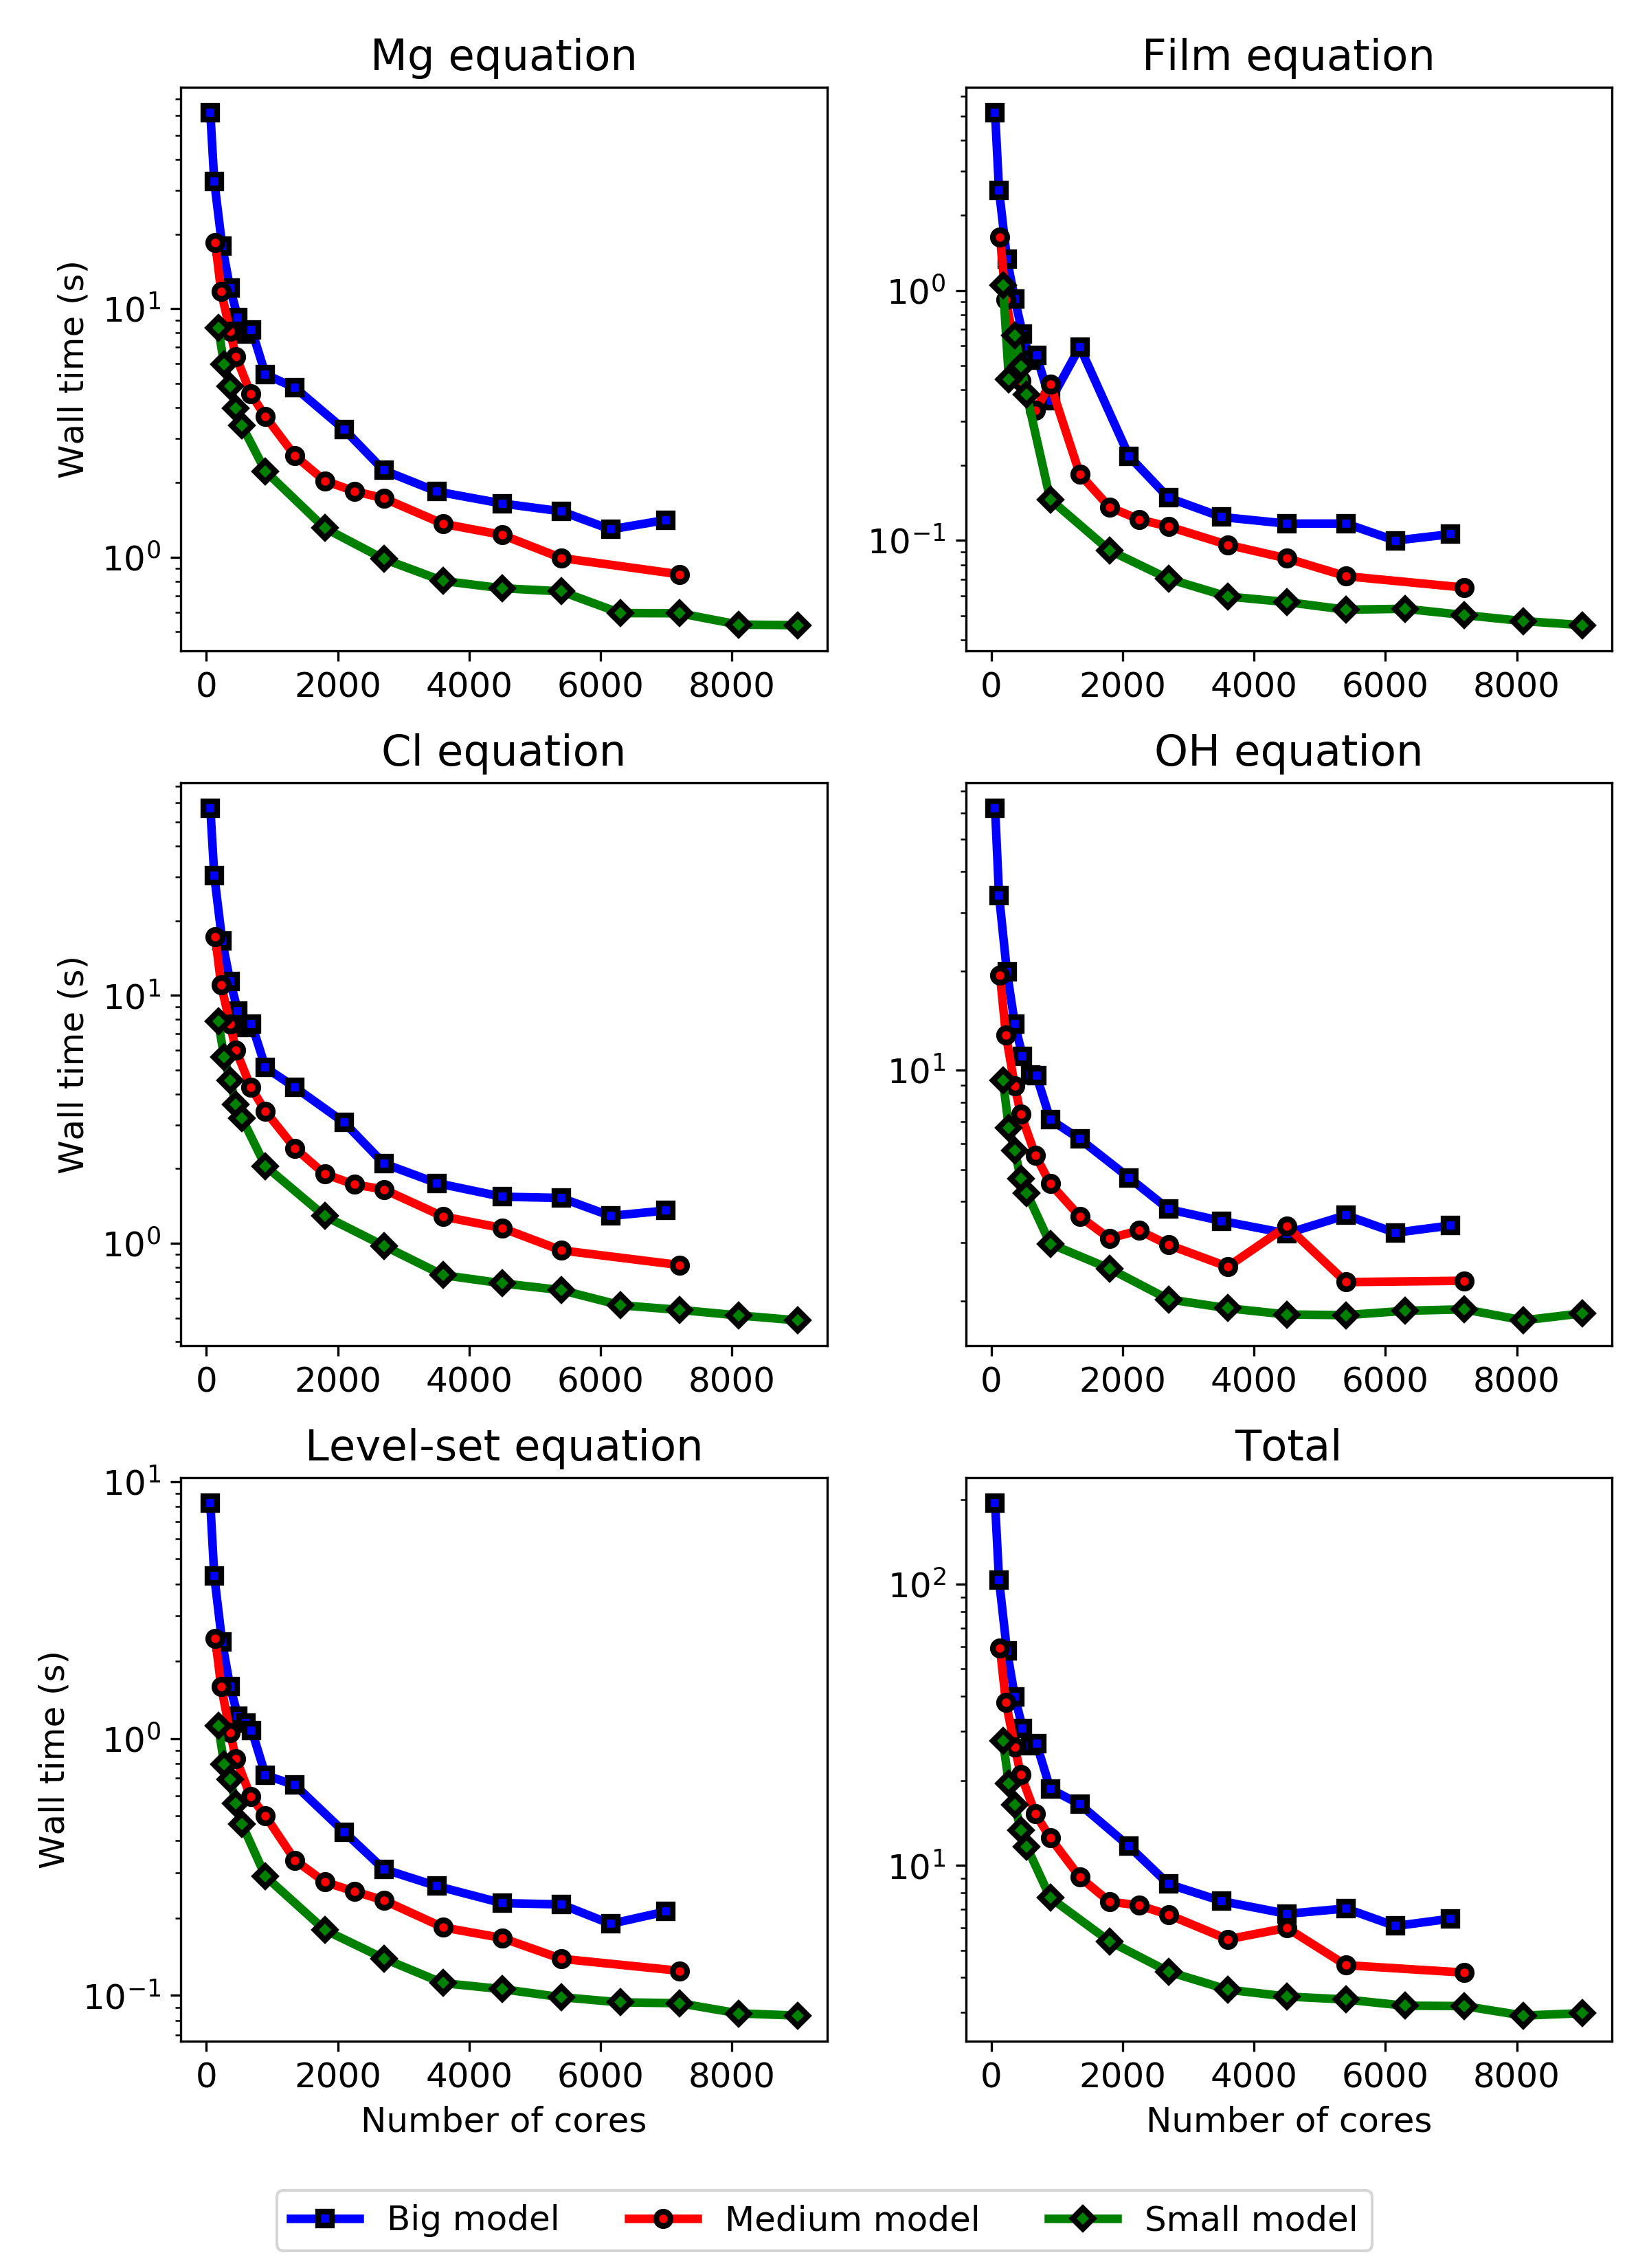
\includegraphics[width=\textwidth]{strong_scaling_vertical.png}
\caption[Strong scaling of individual and combined components of the biodegradation model]{Strong scaling of the computational model, performed using the small, medium, and large mesh for the solution of individual and combined equations of the biodegradation model (Chapter \ref{ch:core}), in which the execution time is plotted in the logarithmic scale versus the varying \gls{CPU} cores.} \label{fig:cup_strong_scaling}
\end{figure}

%\clearpage

As can be seen in the strong scaling results, different \gls{PDE}s show different scaling behavior, the most distinct of which belongs to the OH equation used to calculate the pH change in the surrounding environment. The different scaling behavior is rooted in the boundary conditions used for each equation. They impact the formation of the linear system of equations and appear in the scaling results due to the penalization technique used to implement boundary conditions.

The strong scaling test shows that the optimal size for the distributed computing environment is \num{5000} \gls{CPU} cores, above which no significant improvement in the execution time was observed in all three tested problem sizes. However, the scaling behavior of models slightly differs depending on the size. As expected, in problems with smaller size, the costs associated with inter nodes communication become effective faster in comparison to bigger models, and as a result, increasing the number of nodes becomes useless in earlier stages in these model sizes. This fact can be seen in the cumulative strong scaling plots (the plot in the bottom right), where the graph for the small model tends to reach a vertical line slightly faster in comparison to the graph for the big model.

Fig. \ref{fig:cup_weak_strong} shows the results of the strong and weak scaling tests side by side. As can be seen in the weak scaling result, the model shows an ideal scaling behavior in environments with less than \num{1000} cores. The system shows non-ideal behavior with more \gls{CPU} cores than this, as can be observed in strong scaling results, in which adding more \gls{CPU} cores does not cause a linear drop in the execution time (wall time). The parallel efficiency graphs plotted in Fig. \ref{fig:cup_efficiency} show this behavior more clearly, which are calculated from the strong scaling results.

The weak and strong scaling results clearly indicate that the code can be improved from the performance point of view. Given the current state of \gls{HPC} for biomedical-related simulations and computational modeling works,  even taking 10K \gls{CPU} cores is not unrealistic. The first part of improvement seems to be related to assembling the linear system, in which the schemes used for numerical integration, the order of elements used for various involved physics, and the method for applying boundary conditions play an essential role. Secondly, the configuration of employed preconditioners and iterative solvers can be modified for individual components according to the numerical computing requirements, which can affect their scaling behavior (Fig. \ref{fig:cup_strong_scaling}). However, making a more tangible conclusion on the performance bottlenecks of the developed model requires further analysis of the results for the parallel speedup, similar to the analysis performed in Chapter \ref{ch:hpc} and \cite{Barzegari2022}. Furthermore, it should be taken into account that such performance analysis has an inherent simplification of more complex technical aspects affecting the simulation execution time, such as load balancing, network communication, and per-node limitations in memory access, which may differ in each \gls{HPC} environment due to the configurations made by the system maintainers.

\begin{figure}[h]
\centering
\medskip
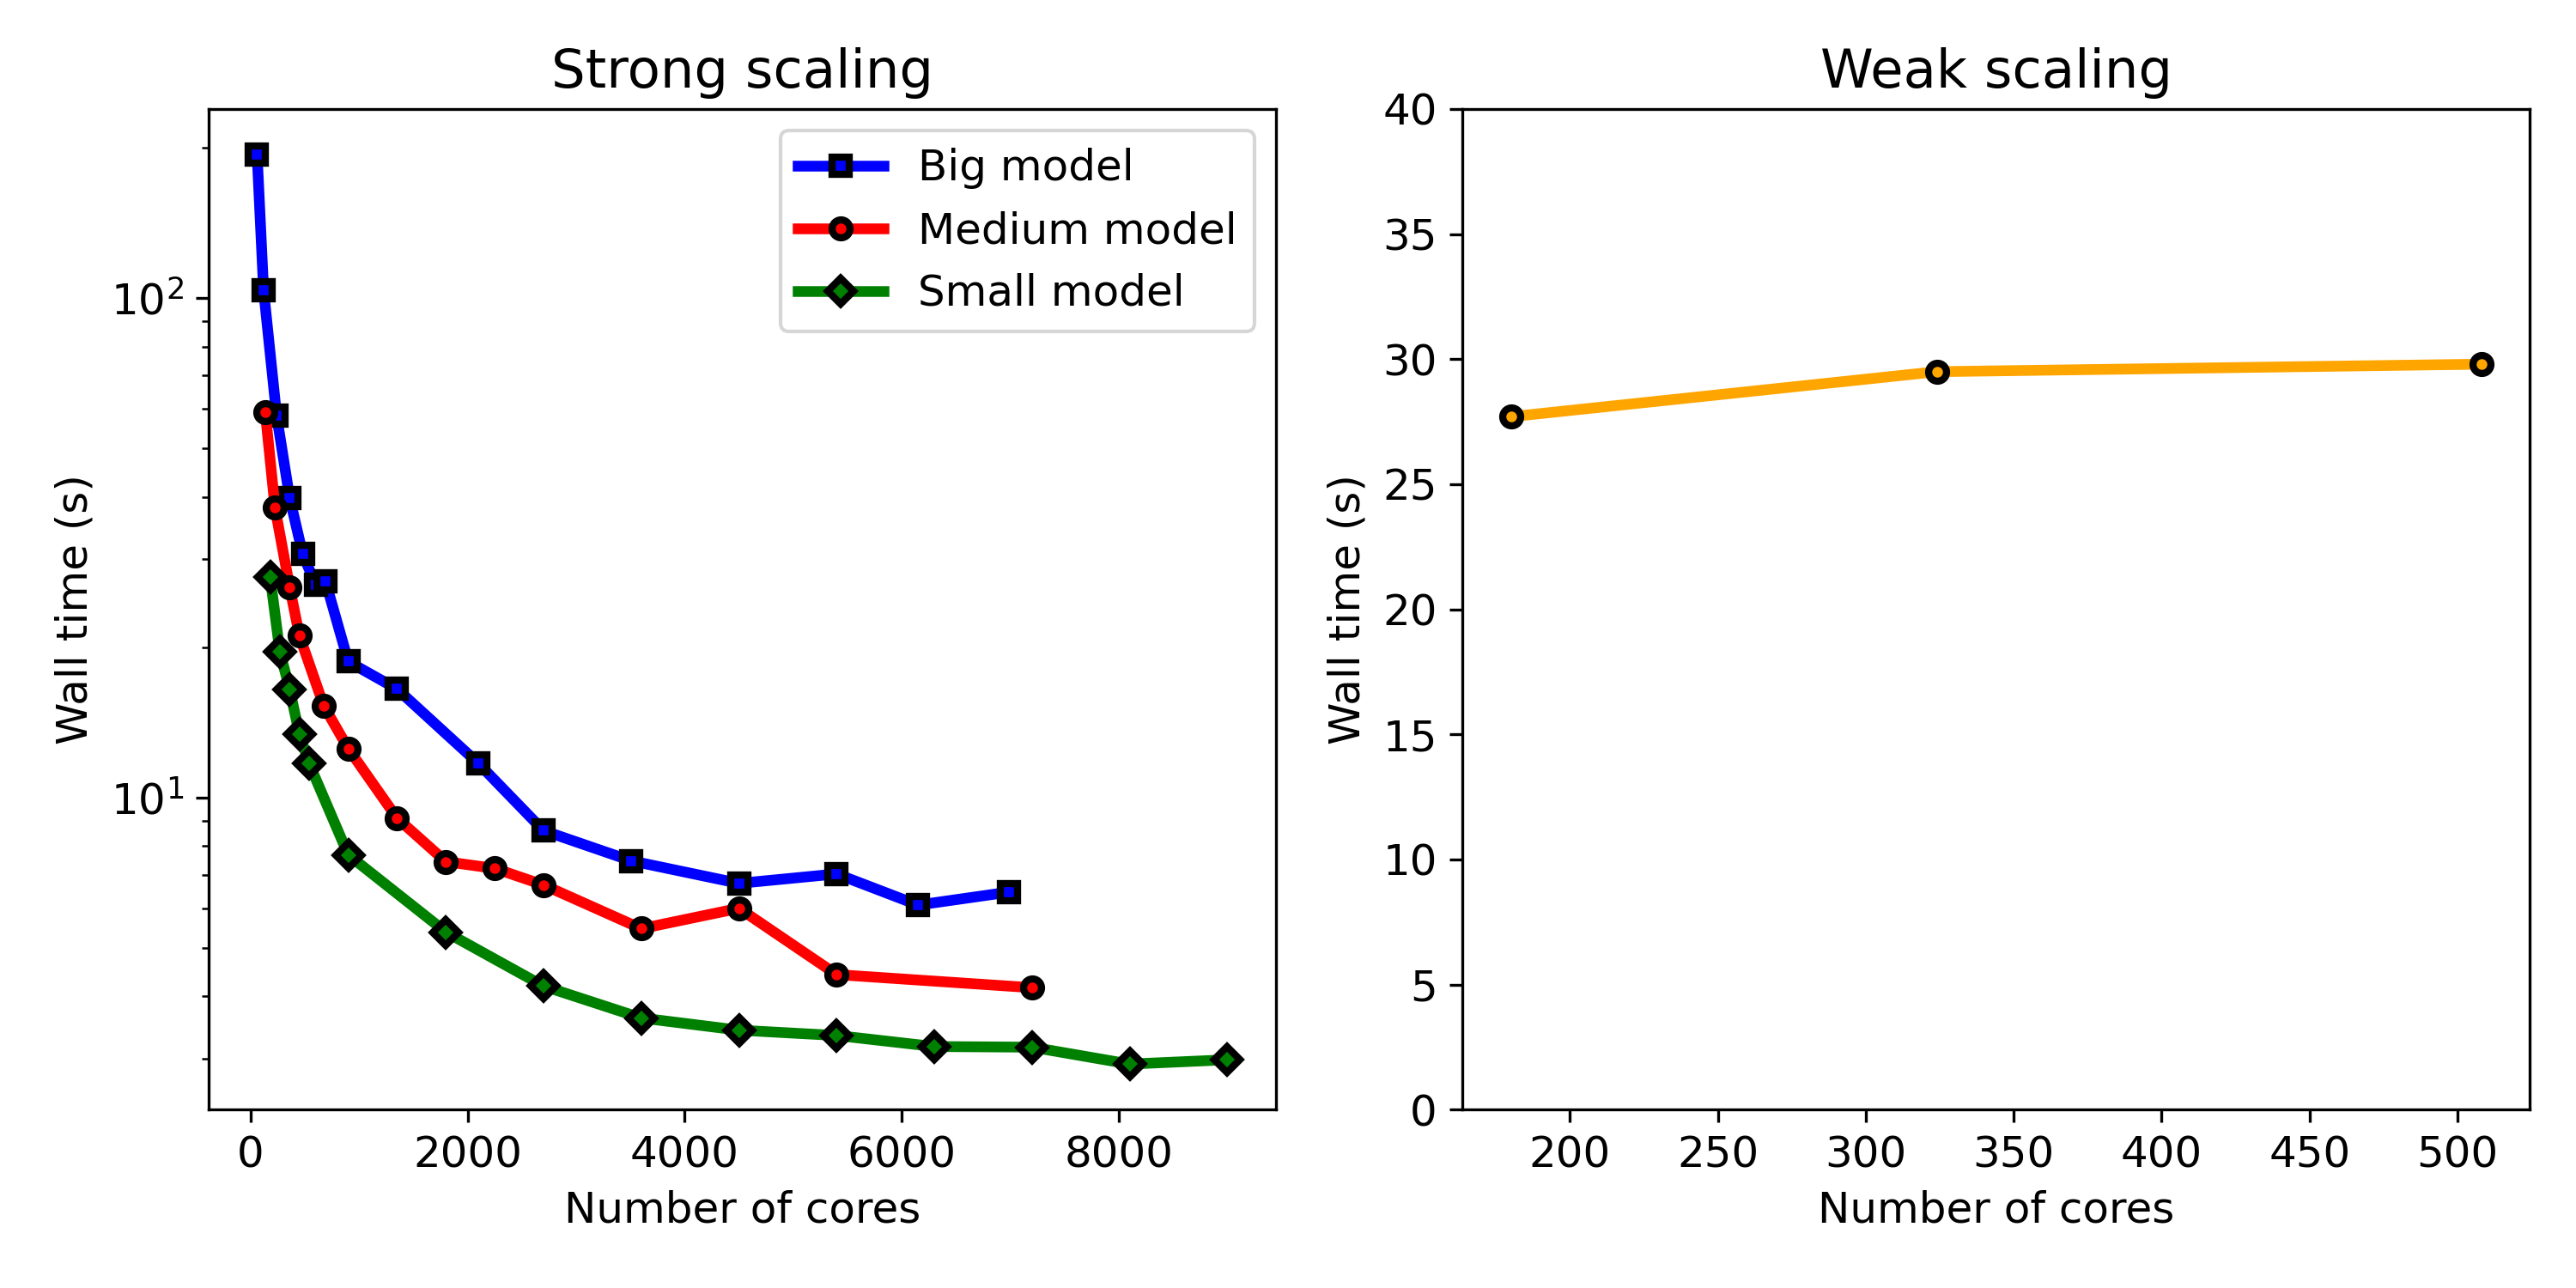
\includegraphics[width=\textwidth]{weak_strong.png}
\caption[Weak and strong scaling of the acetabular implant model]{Weak and strong scaling of the computational biodegradation model of the acetabular implant, plotted for the total time needed to solve all the equations in a single time step.} \label{fig:cup_weak_strong}
\end{figure}

\begin{figure}[h]
\centering
\medskip
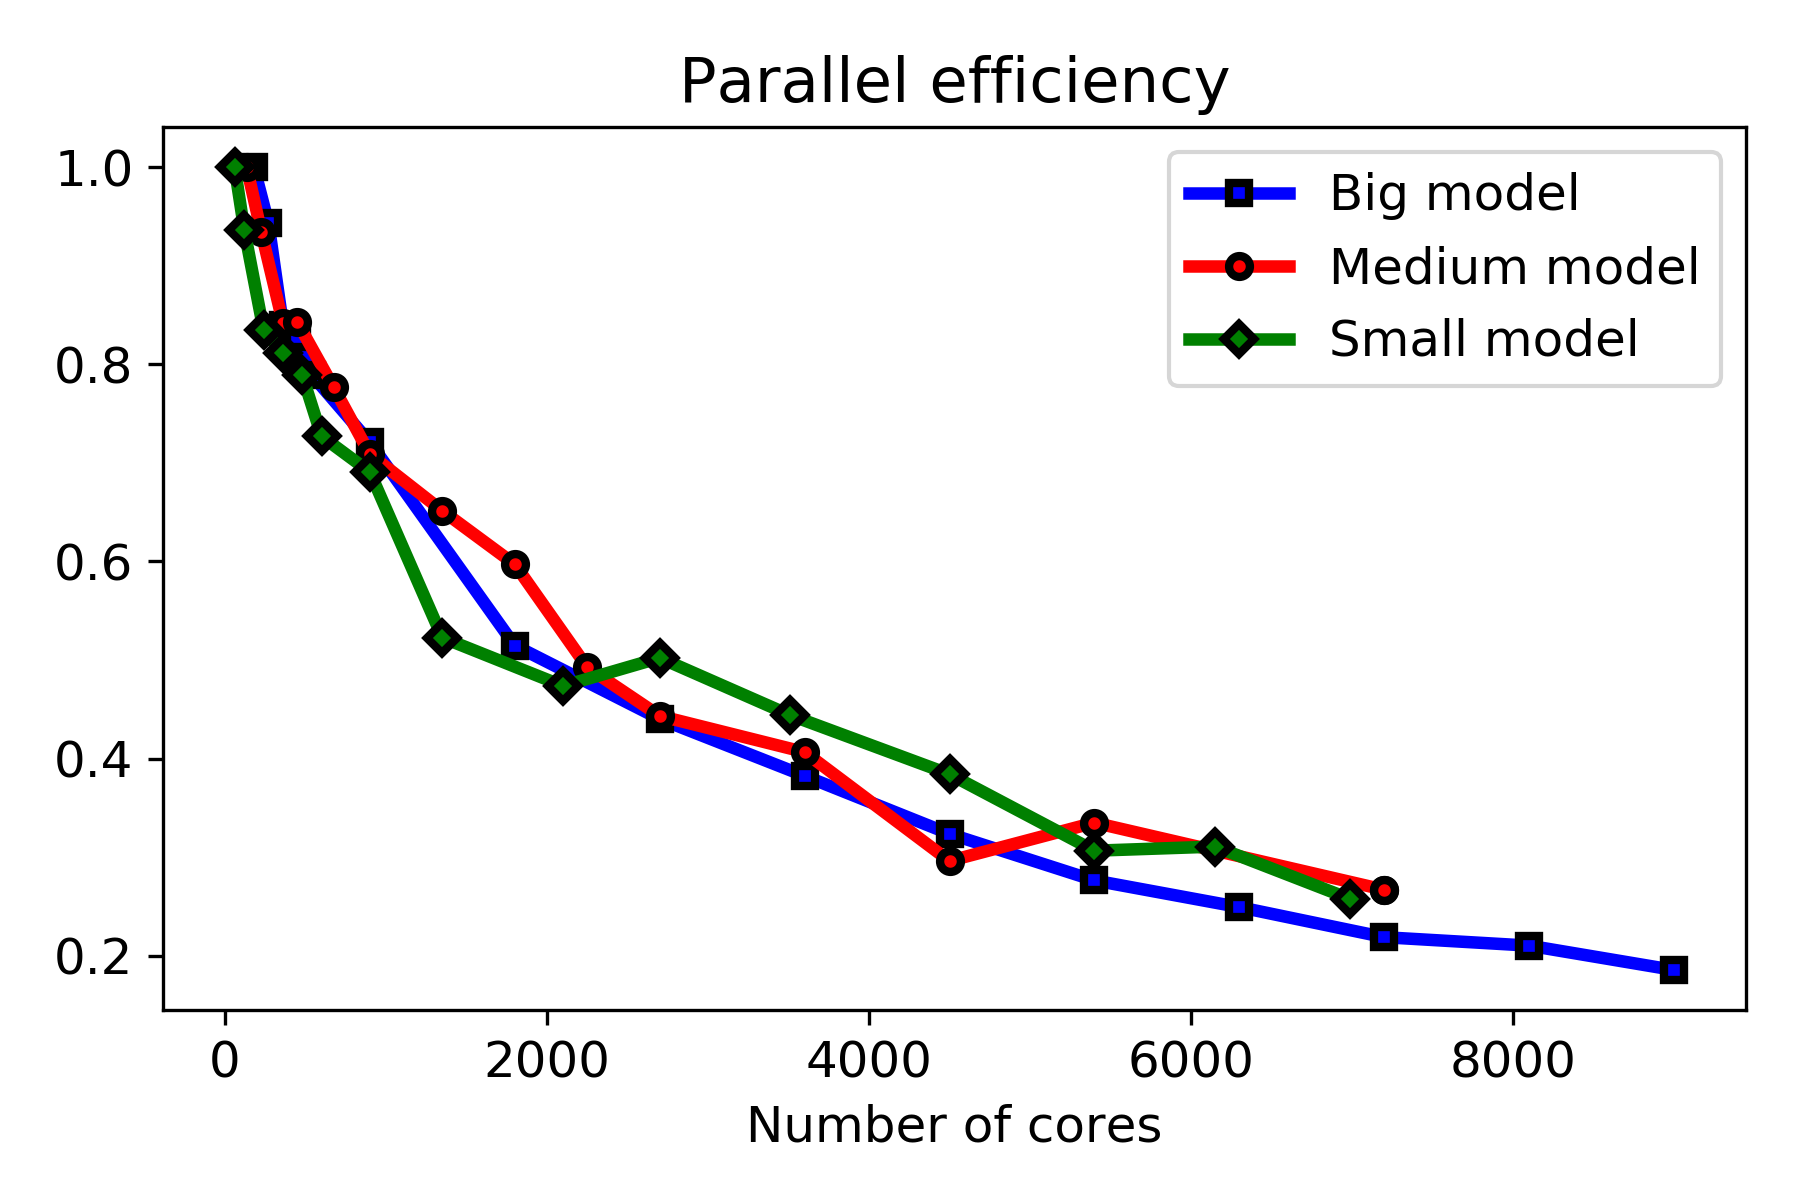
\includegraphics[width=0.7\textwidth]{efficiency.png}
\caption[Parallel efficiency of the acetabular implant model]{Parallel efficiency calculated from the strong scaling results of the computational biodegradation model of the acetabular implant, plotted separately for the small, medium and big models.} \label{fig:cup_efficiency}
\end{figure}


\section{Conclusions}

In this work, taking advantage of \gls{HPC} techniques to simulate a large-scale 3D model led to a computational model capable of predicting the biodegradation behavior of an acetabular implant in high resolution. Results demonstrate the potential of the model to act as a tool for assessing and tuning the biodegradation properties of orthopedic implants regardless of shape or complexity.

\section*{Acknowledgments}

This research is financially supported by the Prosperos project, funded by the Interreg VA Flanders – The Netherlands program, CCI grant no. 2014TC16RFCB046 and by the Fund for Scientific Research Flanders (FWO), grant G085018N. The results were obtained during a research visit to the Computational Science Lab at the University of Amsterdam, funded and supported by FWO long research stay grant V408622N. The computational resources and services used in this work were provided by SURF (www.surf.nl) using the Dutch National Supercomputer Snellius. The visualization works used the ARCHER2 UK National Supercomputing Service (www.archer2.ac.uk).


%%%%%%%%%%%%%%%%%%%%%%%%%%%%%%%%%%%%%%%%%%%%%%%%%%
% Keep the following \cleardoublepage at the end of this file,
% otherwise \includeonly includes empty pages.
\cleardoublepage
